\noindent This chapter will summarize and discuss the results from chapters \ref{chapter:analysis} and \ref{chapter:application}.

\section{Results of verification}
The plots that are discussed in this section can be found in chapter \ref{chapter:analysis}.

\subsection{The FE scheme}
In general, the results from testing the FE implementation are very good. Especially the results from testing the exact numerical solution are informative. 
The numerical exact solution test is a verification of the implementation of the FE scheme. 
A successful test indicates that the scheme is correct and will solve the diffusion equation to the expected accuracy. 
Both the error plots from section \ref{analysis:section_manufactured_solution} and the spatial convergence test are very close to perfect, further suggesting a correct implementation. \\
% While the general convergence tests for the FE scheme could be better (Figure \ref{analysis:convergence_tests:FE}), it is most likely due to other effects. \\
Considering all of the three tests are close to perfect, the FE scheme is deemed correctly implemented within the limits of the applied tests.

\subsection{The BE scheme and the block tridiagonal solver}
Two of the tests done on the BE scheme are slightly off target. 
These are the spatial convergence test and the numerical exact solution. \\
Though the numerical exact solution test is expected to give an error close to machine precision, the results are five orders of magnitude larger than machine precision. 
On the other hand, the error term is also eight orders of magnitude smaller than the time step and there are a lot of possible round-off errors in the inverted coefficient matrix which can explain the lack of accuracy. \\
The spatial convergence test demands that the error associated with the spatial derivative is much larger than the error from the time derivative. 
As the spatial resolution is increased, the spatial error becomes less dominant because the time step is held constant. 
Because the spatial convergence is still clearly larger than one, and starts out at two (which is the value it should converge to), this is considered to be adequate. \\

\noindent Effectively, the manufactured solution test and convergence tests verify the assembly of the coefficient matrix, since an incorrect assembly would produce a larger error term. 
The numerical exact solution test verifies the implementation and accuracy of the block tridiagonal solver, since an incorrectly implemented solver would give results comparable to the numerical exact solution. \\

\noindent In summary, the tests done on the BE scheme verifies that it, and the block tridiagonal solver, are implemented correctly.

\subsection{The RW solver}
Due to fluctuations in the solution it is hard to get a good convergence rate for the RW solver. 
However, it is measured to be close to $0.5$ both with respect to the time step and with respect to the number of walkers introduced. 
% Seeing as there is no exact numerical solution for a random walk, only statistical properties 
The result of verifying the RW solver is that it is deemed correctly implemented within the limits of the applied tests.

\subsection{The hybrid diffusion solver}
For this thesis it is considered very important that the hybrid diffusion solver can have first order convergence in time given a high enough conversion rate. 
As Figure \ref{combined_BE1d:convergence} shows this was achieved, and the hybrid solver is therefore considered adequately implemented for the time being.\\

Effects of varying the relative size of the RW area were also illustrated. 
The result of increasing the portion of the PDE mesh affected by an RW model is clearly a larger error term overall, while decreasing the size of the RW area significantly improves the error term. 
All of this is expected since more fluctuations are introduced by the RW solver.

\section{Results for physical application}

Craske et.al. \cite{craske2005spines} suggest that the neck of spines act as diffusion barriers which slow down, but don't completely stop the diffusion of PKC$\gamma$ into spines. 
The function of this barrier is a bit unclear, but the presence of it is undisputed. 
In their measurements they found a delay of around $5-10$ seconds from elevated concentration levels in the dendrite until a similarly elevated concentration level occurred in spines with necks longer than $0.5\mu$m. 
Using parameter values which resemble the values found in actual (rodent) neurons and neurites in the developed software, the observed delay-times have been recreated. 
Figure \ref{results:spine_diffusion_stats} shows plots of the observed diffusion times into spines. 
This figure shows a clear trend for longer diffusion times as the neck length of the spine increases. 
Figure \ref{results:boxplot_relative_diffusiontime_long_neck} further supports this claim and implies the average diffusion time for PKC$\gamma$ into long necked spines to be in accordance with the results from Craske et.al.
Seeing as there are no additional complexities added to the RW model we can assume that the spine neck does in fact function as a diffusion barrier.
\begin{figure}[h]
 \centering
 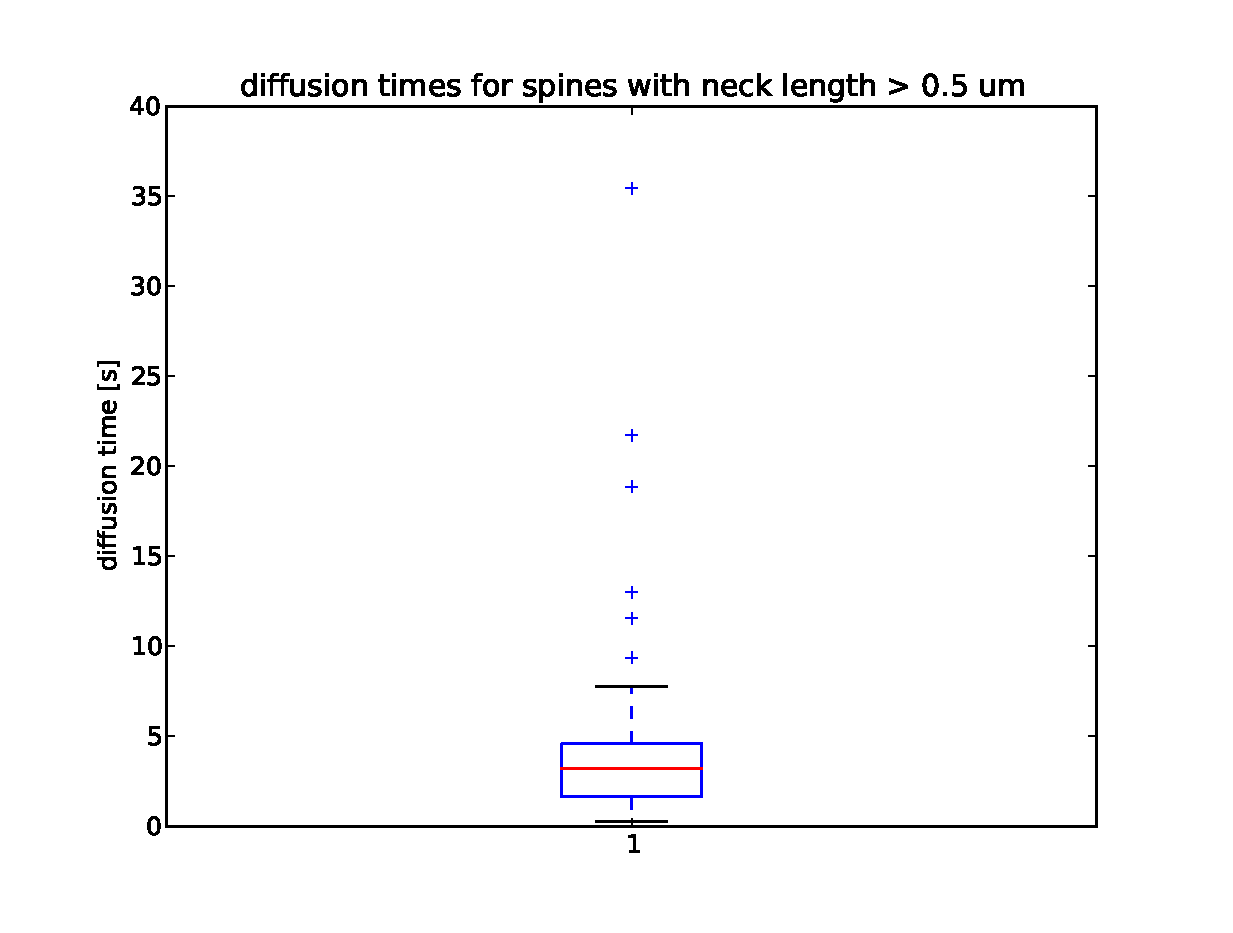
\includegraphics[scale=0.5]{Figures/spine_stats_boxplot_reltime_longneck.eps}
 \caption[Diffusion time for long necked spines]{Boxplot of the relative diffusion times (time between elevated concentration in dendrite and elevated concentration in spine head) into spines with necks longer than $0.5\mu$m. Similar studies were done by Craske et.al. \cite{craske2005spines} and found diffusion time (unclear whether relative or not) to be somewhere around 5-10 seconds.}
 \label{results:boxplot_relative_diffusiontime_long_neck}
\end{figure}

\begin{figure}[h]
 \centering
\begin{subfigure}[b]{0.48\textwidth}
 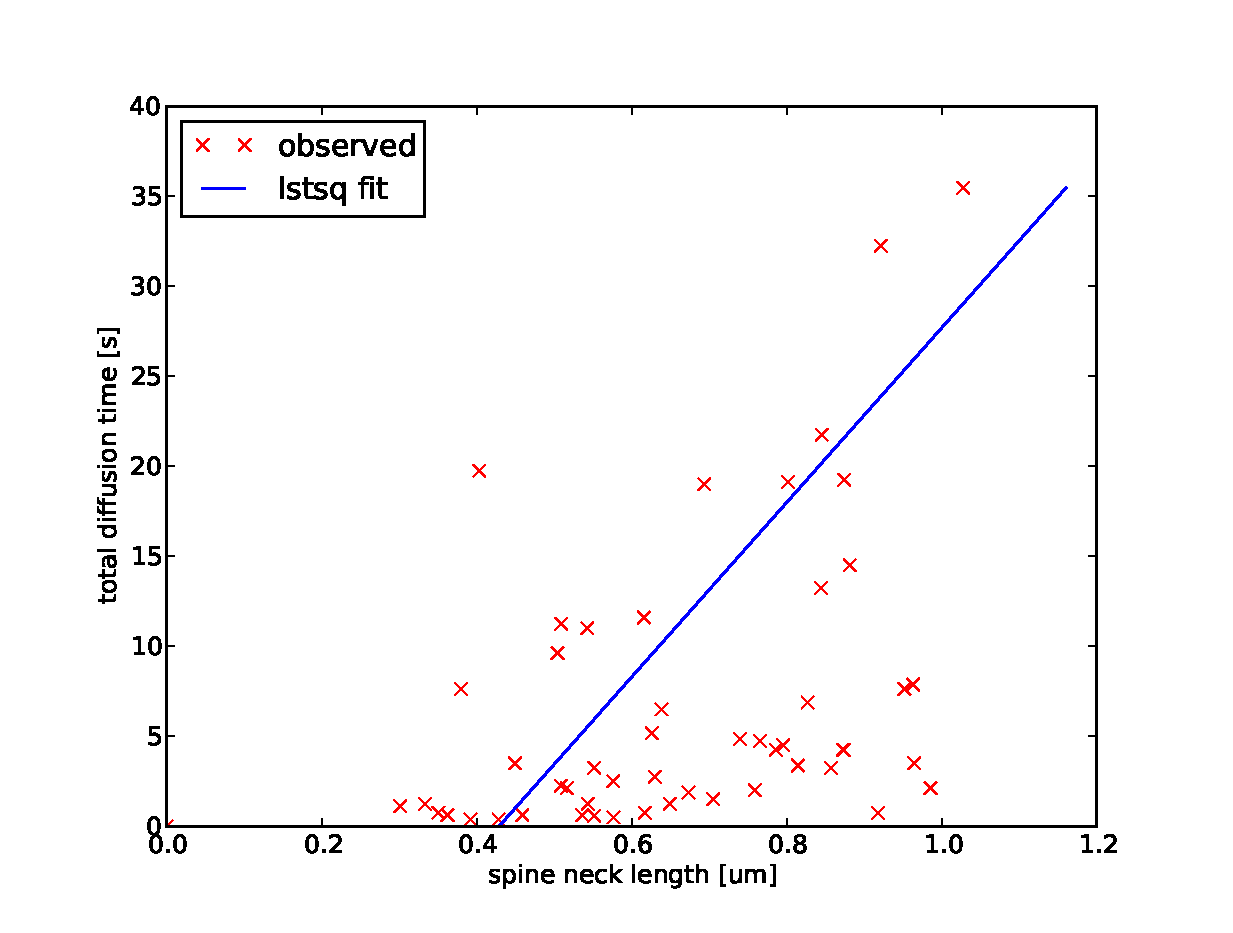
\includegraphics[width=\textwidth]{Figures/spine_stats_fulltime_nl.eps}
 \caption{Absolute diffusion times.}
 \label{results:spine_diffusion_stats:fulltime}
 \end{subfigure}
 \begin{subfigure}[b]{0.48\textwidth}
 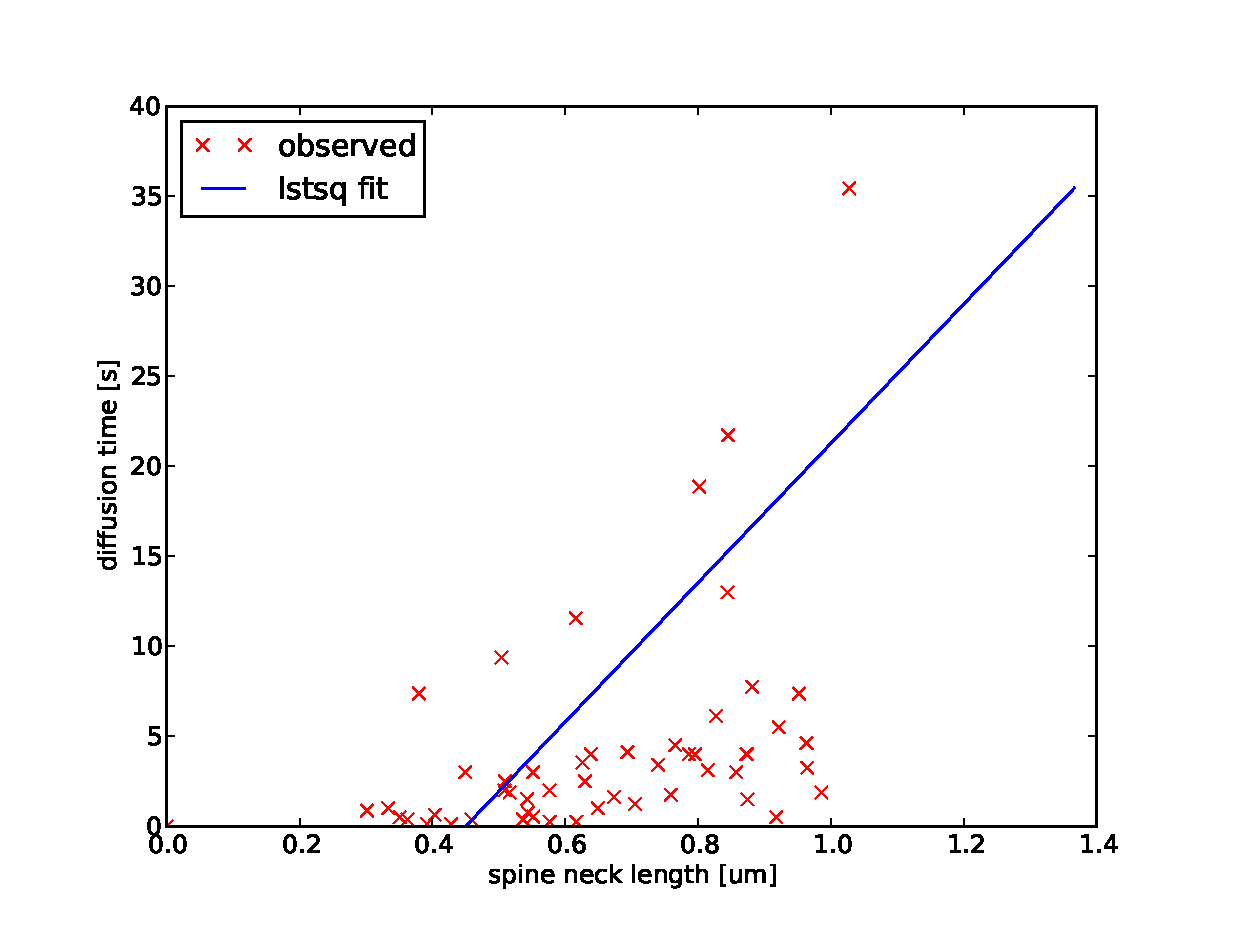
\includegraphics[width=\textwidth]{Figures/spine_stats_reltime_nl.eps}
 \caption{Relative diffusion times.}
 \label{results:spine_diffusion_stats:reltime}
\end{subfigure}
\caption[Diffusion times with least squares fit]{Absolute (a) and relative (b) diffusion times into spines with outliers removed from the data. Outliers are the observations illustrated by crosses in Figure \ref{results:boxplot_relative_diffusiontime_long_neck}. The lines represent a least squares fit of the results. For (a) the least squares fit is $y\approx 0.0346x +0.4424$, where $y$ is the diffusion time and $x$ is the neck length of the spine. For (b) the least squares fit is $y\approx 0.0249x+ 0.4189$. }
\label{results:spine_diffusion_stats}
\end{figure}


Through the simulations it became apparent that there must be some sort of limiting factor which limits the number of PKC$\gamma$ particles that are let into the spine. 
In real life this is achieved by a concentration gradient which tends to zero (or negative values), meaning that no particles will diffuse into the spine after it is ``filled'' up. 
A random walker will not feel this concentration gradient unless it is explicitly told so. 
The alternative solution then, is to reduce the probability for particles to diffuse into a spine for each particle that gets caught in the spine head by a factor $\frac{1}{10}$. 

\section{Using other particle dynamics}

The aim of this project has always been to create a flexible framework where especially the particle dynamics can be substituted. 
A test was therefore executed where Direct Simulation Monte Carlo (\nomenclature{DSMC}{Direct Simulation Monte Carlo}DSMC) code developed by Anders Hafreager for his masters thesis \cite{hafreager2014flow}, was used in stead of the RW model. 
DSMC is a particle dynamics approach where the velocities of individual particles are modeled, but some particle interactions are modeled by a stochastic process. 
Typically, particle collisions are modeled by a Monte Carlo method, but boundary conditions are not.\\

\noindent A problem arises with respect to the coupling described in this thesis: 
In the DSMC model, there is no fixed step length for each particle. It is possible to measure a diffusion coefficient which, to some extent, can be controlled by adjusting the temperature of the system, but this has not been done. 

As a result, this must be viewed as an experiment in which the aim is for the two softwares to communicate as intended. 
In this sense, the experiment was successful. 
Figure \ref{results:anders} shows one time step of a simulation where the DSMC model was used as particle dynamics model. 
As is apparent from the figure, the coupling is not very good. 

\begin{figure}[H]
 \centering
 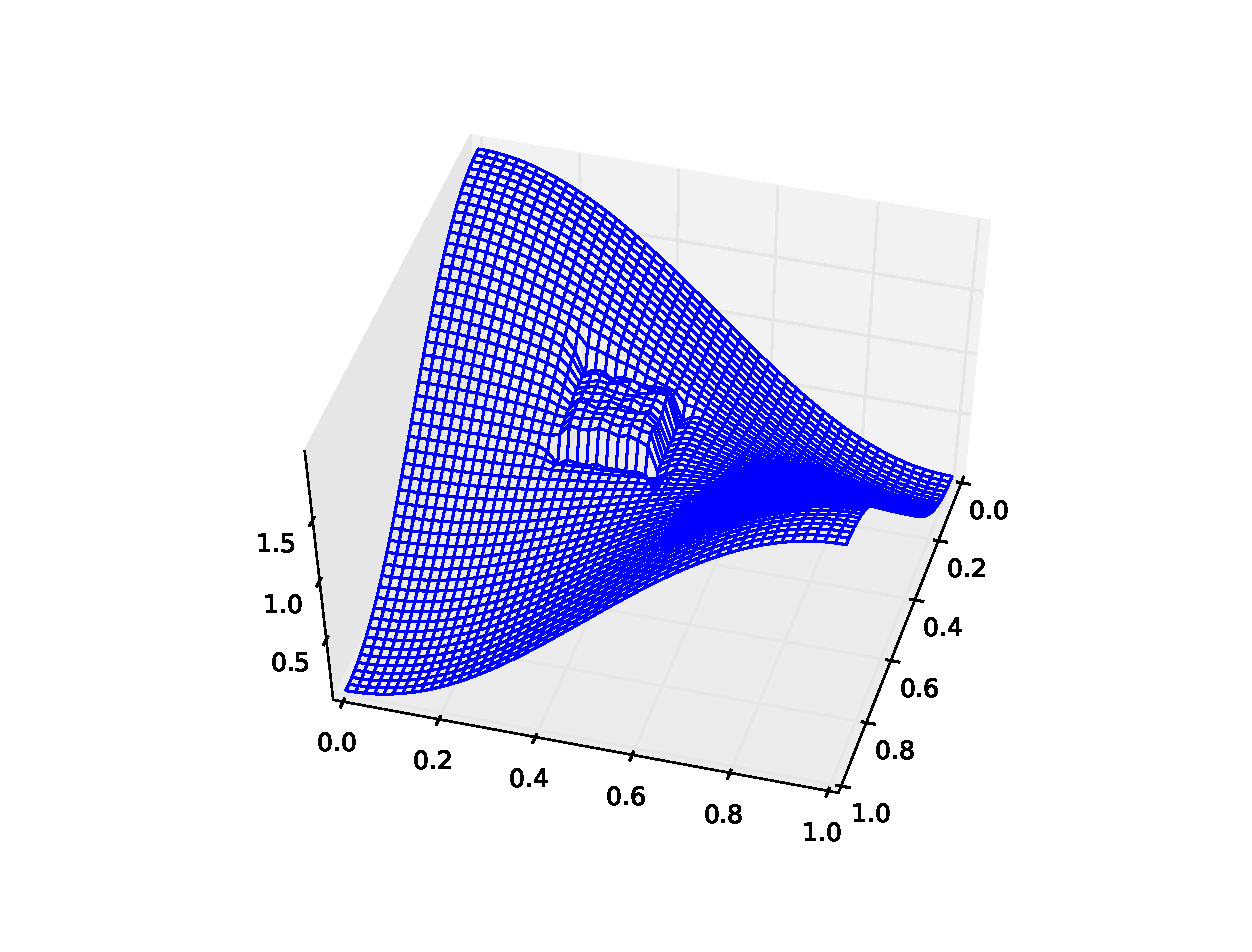
\includegraphics[width=0.7\textwidth]{Figures/anders_stuff.eps}
 \caption[Hybrid solver with DSMC particle model]{This figure shows the hybrid diffusion solver with a DSMC particle model. The coupling between the two modes is not very good, but the communication between them works.}
 \label{results:anders}
\end{figure}
